\documentclass[12pt,a4paper]{article}

% ─── Paquetes ────────────────────────────────────────────────────────────────
\usepackage[a4paper, top=2.5cm, bottom=2.5cm, left=2.5cm, right=2.5cm]{geometry}
\usepackage[spanish]{babel}
\usepackage{amsmath}
\usepackage{amssymb}
\usepackage{booktabs}
\usepackage{graphicx}
\usepackage[hidelinks]{hyperref}
\usepackage{xcolor}
\usepackage{array}
\usepackage{longtable}
\usepackage{multirow}
\usepackage{float}
\usepackage{caption}
\usepackage{fancyhdr}
\usepackage{parskip}
\usepackage{tikz}
\usetikzlibrary{arrows.meta,positioning,babel}
\usepackage{pgfplots}
\pgfplotsset{compat=1.18}
\usepackage{pgfplotstable}
\usepackage{colortbl}
\usepackage{tabularx}
\usepackage{makecell}

% ─── Enunciado box ───────────────────────────────────────────────────────────
\newcommand{\enunciado}[1]{}

% ─── Configuración general ───────────────────────────────────────────────────
\setlength{\parindent}{0pt}
\setlength{\headheight}{15pt}
\setlength{\parskip}{6pt}

% ─── Encabezado / pie de página ──────────────────────────────────────────────
\pagestyle{fancy}
\fancyhf{}
\renewcommand{\headrulewidth}{0.4pt}
\fancyhead[L]{\small\textsc{Gestión de Operaciones}}
\fancyhead[R]{\small\textsc{Tarea 3 — Grupo 3}}
\fancyfoot[C]{\thepage}

% ─────────────────────────────────────────────────────────────────────────────
\begin{document}

% ════════════════════════════════════════════════════════════════════════════
%  PORTADA
% ════════════════════════════════════════════════════════════════════════════
\thispagestyle{empty}

% --- Franja superior: logo + nombre institución ----------------------------
\noindent
\begin{minipage}[c]{0.12\textwidth}
    
\includegraphics[width=2cm]{logo_uc-000.png}
\end{minipage}%
\hfill
\begin{minipage}[c]{0.84\textwidth}
    \raggedleft
    {\small\textsc{Pontificia Universidad Católica de Chile}}\\[2pt]
    {\small\textsc{Escuela de Ingeniería}}
\end{minipage}

\vspace{4pt}
\noindent\rule{\linewidth}{0.8pt}

% --- Cuerpo central --------------------------------------------------------
\vspace{4cm}

\begin{center}
    {\Huge\bfseries Tarea 3}\\[0.6cm]
    {\large Variabilidad, Centros de Distribución y Calidad}
\end{center}

\vfill

% --- Tabla de información --------------------------------------------------
\noindent
\begin{tabular}{@{} >{\bfseries}p{4.2cm} p{10cm} @{}}
    \toprule
    Sección   & Sección 1 \\
    \midrule
    Grupo     & Grupo 3 \\
    \midrule
    Integrantes
              & Ignacio Henríquez \\
              & César Meneses \\
              & Fabián Ortega \\
              & Diego Pérez \\
              & José Manuel Valdés \\
    \midrule
    Trabajo   & Tarea 3 --- Variabilidad, Centros de Distribución y Calidad \\
    \midrule
    Profesor  & Alejandro Mac Cawley \\
    Curso     & Gestión de Operaciones \\
    \midrule
    Fecha     & 22 de junio de 2026 \\
    \bottomrule
\end{tabular}

\newpage

% ════════════════════════════════════════════════════════════════════════════
%  PREGUNTAS
% ════════════════════════════════════════════════════════════════════════════

\section*{Pregunta 1: Variabilidad (40 puntos)}
\setcounter{section}{1}\setcounter{subsection}{0}

\subsection*{1. Diagrama del proceso}

A continuación se presenta el diagrama del proceso de recepción y control de calidad de la fruta, con las respectivas capacidades en cada etapa.

\begin{figure}[H]
    \centering
    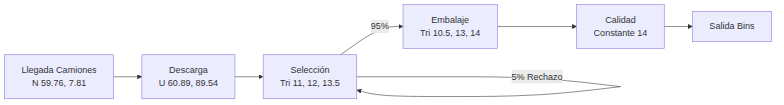
\includegraphics[width=0.9\textwidth]{p1/diagrama_p1.png}
    \caption{Diagrama de flujo del proceso.}
\end{figure}

\subsection*{2. Distribución de llegada}

El tiempo entre llegadas de los camiones se modela como una distribución Normal, y la descarga como una distribución Uniforme, de acuerdo con la validación de datos.

\subsection*{3. Resultados de simulación: utilización y tiempos}

\subsection*{4. Identificación del cuello de botella}

\subsection*{5. Multas por pérdida de calidad}

\subsection*{6. Ubicación del control de calidad}

\subsection*{7. Reducción de variabilidad (Selección vs Embalaje)}

\subsection*{8. Cambios en un mes de funcionamiento}


\newpage
\section*{Pregunta 2: Centro de distribución y diseño de bodega (50 puntos)}
\setcounter{section}{2}\setcounter{subsection}{0}

\subsection*{1. Rotación anual por cámara}

\subsection*{2. Cantidad mínima de operadores}

\subsection*{3. Costo total mensual}

\subsection*{4. Tasa de servicio}

\subsection*{5. Nivel factible de apilamiento y superficie mínima}

\subsection*{6. Frecuencia de reabastecimiento por SKU}

\subsection*{7. Profundidad óptima de almacenamiento}

\subsection*{8. Diseño gráfico de la cámara}

\begin{figure}[H]
    \centering
    % \includegraphics[width=0.8\textwidth]{p2/diseno_camara.png}
    \caption{Diseño de la cámara con pasillo compartido y profundidad óptima.}
\end{figure}

\subsection*{9. Eficiencia de uso del espacio}

\subsection*{10. Beneficio del pickeo frontal}

\subsection*{11. Asignación de posiciones de pickeo}


\newpage
\section*{Pregunta 3: Control de calidad y capacidad de procesos (30 puntos)}
\setcounter{section}{3}\setcounter{subsection}{0}

\subsection*{1. Riesgo del proveedor y de Vertiente Andina}

\subsection*{2. Cartas de control del proceso}

\begin{figure}[H]
    \centering
    % \includegraphics[width=0.8\textwidth]{p3/carta_control.png}
    \caption{Cartas de control para vigilar el nivel promedio y la variabilidad.}
\end{figure}

\subsection*{3. Capacidad del proceso y metodología DMAIC}

\subsection*{4. Proceso mejorado y nueva capacidad}

\begin{figure}[H]
    \centering
    % \includegraphics[width=0.8\textwidth]{p3/grafico_capacidad.png}
    \caption{Distribución del proceso mejorado junto con límites de especificación.}
\end{figure}

\subsection*{5. Impacto económico y costo esperado del despacho}


\end{document}
